% Provenance (never printed): see sources/outline_sources.md (Year 2: metamorphic reactions,
% Clapeyron slopes, the Al2SiO5 diagram, the facies grid, protoliths). Definitions and facies
% table from the IUGS subcommission proposal (via the Granada translation); thermodynamic data
% from Robie and Hemingway (1995); experimental diagram from Holdaway and Mukhopadhyay (1993);
% curves from figdata/bachelor-2/facies.py; exercise and problem values in the Book 4 scratch
% calculator calc/ch10.py.
\chapter{कायांतरी अभिक्रियाएँ और संलक्षणियाँ}\label{ch:b2:metamorphic-facies}

अपनी प्लेट के साथ धँसने वाला बेसाल्ट बेसाल्ट नहीं रहता। उसके प्लैजियोक्लेज़ और पाइरॉक्सीन
ठोस अवस्था में अभिक्रिया करके दूसरे खनिज बनाते हैं, और नया समुच्चय उस
दाब और तापमान पर निर्भर करता है जहाँ तक वह पहुँचा: ग्लॉकोफ़ेन और लॉसनाइट की एक नीली चट्टान, या
ओम्फ़ैसाइट और गार्नेट की एक हरी-लाल चट्टान। कायांतरित चट्टानें सतह पर लौटने पर ये खनिज
बनाए रखती हैं, और अभिक्रियाओं को जानने वाला शैलिकीविद
परिस्थितियों को वापस पढ़ सकता है। यह अध्याय उन अभिक्रियाओं को रसायन-विज्ञान के पाठ्यक्रम के
ऊष्मागतिकी से लिखता है, मापे गए आँकड़ों से सबसे प्रसिद्ध कायांतरी प्रावस्था आरेख परिकलित करता है,
यानी तीन \ce{Al2SiO5} खनिजों का आरेख, उसकी तुलना प्रयोग से करता है, और
कायांतरित चट्टानों के समुच्चयों को संलक्षणियों में व्यवस्थित करता है।
% ledger: scmr:facies-assemblages

\begin{recall}
\textbf{पुस्तक 2 (उच्च माध्यमिक) से}: \omterm{def:b2:metamorphic-facies:metamorphism}{कायांतरण}, \omterm{def:b2:metamorphic-facies:metamorphism}{कायांतरण} श्रेणी, सूचक खनिज
और समश्रेणी-रेखाएँ, संपर्क \omterm{def:b2:metamorphic-facies:metamorphism}{कायांतरण} और उसका परिमंडल, पर्णन और शिस्टता,
शैलस्थैतिक दाब; बहुरूपों के रूप में कायनाइट, ऐंडालुसाइट और सिलिमेनाइट, और उनका
प्रावस्था आरेख। \textbf{भौतिकी और रसायन-विज्ञान की पुस्तकों (प्रथम वर्ष) से}: गिब्स
ऊर्जा $G = H - TS$, जिसका न्यूनतम दिए गए $T$ और $P$ पर स्थायी अवस्था बताता है;
एन्थैल्पी, एन्ट्रॉपी और ऊष्मा धारिता; $\mathrm dG = V\,\mathrm dP - S\,\mathrm dT$; किसी शुद्ध पदार्थ के
वाष्पन के लिए क्लॉसियस--क्लेपेरॉन संबंध और जल का त्रिक
बिंदु। \textbf{पुस्तक 3 (स्नातक वर्ष 1) से}: क्षेपण क्षेत्र, टक्कर-पट्टियाँ और
जियोथर्म।
\end{recall}

\section{कायांतरण}\label{sec:b2:metamorphic-facies:metamorphism}

पुस्तक 2 में \omterm{def:b2:metamorphic-facies:metamorphism}{कायांतरण} से भेंट ऊष्मा और दाब द्वारा चट्टान के रूपांतरण के रूप में हुई थी।
एक अंतरराष्ट्रीय अनुशंसा वह परिभाषा देती है जो यहाँ प्रयुक्त होती है।

\begin{definition}[कायांतरण; प्रोटोलिथ]\label{def:b2:metamorphic-facies:metamorphism}
\emph{कायांतरण}\index{कायांतरण} वह प्रक्रम है जो किसी चट्टान के खनिजों या
सूक्ष्म-संरचना, या दोनों, को मुख्यतः ठोस अवस्था में बदलता है, जब चट्टान ऐसी भौतिक परिस्थितियों के
अनुरूप ढलती है जो उन परिस्थितियों से भिन्न हैं जिनमें वह बनी थी, और उनसे भी जो
पृथ्वी की सतह पर और डायाजेनेसिस के क्षेत्र में सामान्यतः पाई जाती हैं। यह
\omterm{def:b2:mantle-melting:melting}{आंशिक गलन} के साथ हो सकता है और चट्टान का रासायनिक संघटन बदल सकता है। कायांतरण से पहले की
चट्टान उसका \emph{प्रोटोलिथ}\index{प्रोटोलिथ} है।
\end{definition}
% ledger: scmr:metamorphism

निचली सीमा डायाजेनेसिस को, यानी किसी अवसाद के दबने और शिलीभूत होने के साथ होने वाले परिवर्तनों को,
बाहर रखती है, और ऊपरी सीमा गलन है, जिसका अध्ययन \cref{ch:b2:crustal-melting} में होता है।
कारक हैं तापमान, दाब, चट्टान से होकर परिसंचरित होने वाले तरल (सबसे बढ़कर जल और
कार्बन डाइऑक्साइड) और विरूपण। \omterm{def:b2:metamorphic-facies:metamorphism}{कायांतरण} का वर्गीकरण उसके विस्तार और
उसके परिवेश से होता है।
% ledger: scmr:metamorphism, scmr:types

\emph{क्षेत्रीय} \omterm{def:b2:metamorphic-facies:metamorphism}{कायांतरण} चट्टान के बड़े आयतनों को प्रभावित करता है और बड़े पैमाने की
विवर्तनिक प्रक्रियाओं के साथ होता है: पर्वत-पट्टियों में, जहाँ टक्कर में भूपर्पटी मोटी होती है, यह \emph{पर्वतजनक} होता है;
\emph{दफ़न} \omterm{def:b2:metamorphic-facies:metamorphism}{कायांतरण} उन चट्टानों को प्रभावित करता है जो मोटे अवसादी या ज्वालामुखीय ढेरों के नीचे गहराई तक दबी हैं,
विरूपण या मैग्मावाद के बिना, जिससे उसकी चट्टानों में
सामान्यतः शिस्टता नहीं होती; \emph{महासागर-तल} \omterm{def:b2:metamorphic-facies:metamorphism}{कायांतरण} प्रसारी कटकों के निकट भूपर्पटी को
बदलता है, जहाँ गरम समुद्री जल तीव्र ऊष्मीय प्रवणताओं के अधीन उसमें से होकर परिसंचरित होता है,
और उसका पुनःक्रिस्टलन सामान्यतः अपूर्ण रहता है। \emph{स्थानीय} \omterm{def:b2:metamorphic-facies:metamorphism}{कायांतरण}
का कारण स्थानीय होता है: \emph{संपर्क} \omterm{def:b2:metamorphic-facies:metamorphism}{कायांतरण} किसी अंतर्वेधन की आतिथेय चट्टानों को गरम करता है;
\emph{जलतापीय} \omterm{def:b2:metamorphic-facies:metamorphism}{कायांतरण} गरम, जल-समृद्ध तरलों से चलता है;
भ्रंश और अपरूपण क्षेत्रों में \emph{विस्थापन} \omterm{def:b2:metamorphic-facies:metamorphism}{कायांतरण} कण-आकार घटाता है और
मायलोनाइट तथा कैटाक्लासाइट बनाता है; \omterm{def:b2:planet-formation-meteorites:fall-find}{उल्कापिंड} के प्रभाव के नीचे \emph{आघात} \omterm{def:b2:metamorphic-facies:metamorphism}{कायांतरण}
चट्टान को पिघला और वाष्पित कर सकता है। तापमान बढ़ते समय \omterm{def:b2:metamorphic-facies:metamorphism}{कायांतरण} को प्रगामी कहते हैं और
घटते समय प्रतिगामी।
% ledger: scmr:types

\section{कायांतरी अभिक्रियाएँ}\label{sec:b2:metamorphic-facies:reactions}

\begin{definition}[कायांतरी अभिक्रिया; वाष्पशील-निष्कासन अभिक्रिया]\label{def:b2:metamorphic-facies:reaction}
\emph{कायांतरी अभिक्रिया}\index{कायांतरी अभिक्रिया} किसी चट्टान के खनिजों के एक समुच्चय,
अभिकारकों, को ठोस अवस्था में दूसरे समुच्चय, उत्पादों, में बदलती है, संभवतः
किसी तरल प्रावस्था की भागीदारी के साथ। \emph{वाष्पशील-निष्कासन अभिक्रिया}\index{वाष्पशील-निष्कासन अभिक्रिया}
वह है जो कोई वाष्पशील मुक्त करती है: निर्जलीकरण अभिक्रिया में जल, या विकार्बनीकरण अभिक्रिया में कार्बन
डाइऑक्साइड।
\end{definition}

इस अध्याय में तीन प्रकार आएँगे। बहुरूपी परिवर्तन, जैसे कायनाइट से
सिलिमेनाइट या कैल्साइट से ऐरागोनाइट, सूत्र बनाए रखते हैं और संरचना बदलते हैं।
ठोसों के बीच अन्य अभिक्रियाएँ खनिजों के बीच घटकों का पुनर्वितरण करती हैं, जैसे
एल्बाइट से जेडाइट और क्वार्ट्ज़ बनना:
\[
\ce{NaAlSi3O8 -> NaAlSi2O6 + SiO2}.
\]
वाष्पशील-निष्कासन अभिक्रियाएँ कोई तरल मुक्त करती हैं, जैसे उच्च तापमान पर मस्कोवाइट और क्वार्ट्ज़ का
विघटन:
\[
\ce{KAl3Si3O10(OH)2 + SiO2 -> KAlSi3O8 + Al2SiO5 + H2O}.
\]
% ledger: day73:ms-qz

स्थिर संघटन वाले खनिजों के बीच अभिक्रिया के लिए गिब्स ऊर्जा का परिवर्तन
$\Delta_r G(T, P) = \sum G_{\text{उत्पाद}} - \sum G_{\text{अभिकारक}}$ है; उत्पाद
वहाँ स्थायी हैं जहाँ $\Delta_r G < 0$, अभिकारक वहाँ जहाँ $\Delta_r G > 0$, और दोनों
वहाँ सहअस्तित्व में होते हैं जहाँ $\Delta_r G = 0$।

\begin{definition}[एकचरी अभिक्रिया]\label{def:b2:metamorphic-facies:univariant}
स्थिर संघटन वाली प्रावस्थाओं के बीच अभिक्रिया \emph{एकचरी}\index{एकचरी अभिक्रिया}
होती है जब उसकी साम्य-शर्त $\Delta_r G(T, P) = 0$ एक चर को
मुक्त छोड़ती है: साम्य दाब--तापमान तल में एक रेखा है, जो
अभिकारकों के क्षेत्र को उत्पादों के क्षेत्र से अलग करती है।
\end{definition}

\begin{definition}[क्लेपेरॉन ढलान]\label{def:b2:metamorphic-facies:clapeyron}
किसी अभिक्रिया की \emph{क्लेपेरॉन ढलान}\index{क्लेपेरॉन ढलान} दाब--तापमान तल में
उसकी साम्य-रेखा की ढलान $\mathrm dP/\mathrm dT$ है।
\end{definition}

\begin{proposition}[किसी अभिक्रिया की क्लेपेरॉन ढलान]\label{prop:b2:metamorphic-facies:clapeyron}
एन्ट्रॉपी परिवर्तन $\Delta_r S$ और आयतन
परिवर्तन $\Delta_r V$ वाली अभिक्रिया की साम्य-रेखा के अनुदिश,
\[
\frac{\mathrm dP}{\mathrm dT} = \frac{\Delta_r S}{\Delta_r V}.
\]
\end{proposition}

\begin{proof}
हर प्रावस्था के लिए $\mathrm dG = V\,\mathrm dP - S\,\mathrm dT$, अतः अभिक्रिया के लिए
$\mathrm d(\Delta_r G) = \Delta_r V\,\mathrm dP - \Delta_r S\,\mathrm dT$। रेखा के अनुदिश
$\Delta_r G = 0$ शून्य ही रहता है: $\Delta_r V\,\mathrm dP = \Delta_r S\,\mathrm dT$।
\end{proof}

यह भौतिकी का क्लॉसियस--क्लेपेरॉन संबंध है, ठोसों के लिए लिखा गया।
$\Delta_r S$ को \unit{J.mol^{-1}.K^{-1}} में और $\Delta_r V$ को \unit{J.bar^{-1}} में लेने पर (एक
\unit{J.bar^{-1}} \qty{10}{cm^3} है), ढलान बार प्रति केल्विन में आती है। दो
परिणाम हर कायांतरी प्रावस्था आरेख को आकार देते हैं। ठोसों के बीच एन्ट्रॉपी और आयतन के
परिवर्तन छोटे होते हैं, जिससे कोई अभिक्रिया-रेखा तीव्र या मंद, धनात्मक या
ऋणात्मक हो सकती है: उच्च-तापमान ओर अधिक एन्ट्रॉपी वाले उत्पाद रखती है, और
उच्च-दाब ओर कम आयतन वाले। \omterm{def:b2:metamorphic-facies:reaction}{वाष्पशील-निष्कासन अभिक्रिया} में तरल
बड़ी एन्ट्रॉपी लाता है, अतः उत्पाद उच्च-तापमान ओर स्थित होते हैं; और तरल का आयतन,
जो निम्न दाब पर बड़ा होता है और दाब बढ़ने के साथ सिकुड़ता है, ढलान को
निम्न दाब पर मंद और उच्च दाब पर अधिक तीव्र बनाता है। अभिक्रिया-रेखा मुड़ती है।
मस्कोवाइट और क्वार्ट्ज़ पर प्रयोग इसे 1,
2 और \qty{3}{kbar} जल-दाब पर 603, 637 और \qty{662}{\celsius} पर रखते हैं: 1 और \qty{2}{kbar} के बीच रेखा
प्रति केल्विन \qty{29}{bar} चढ़ती है, 2 और 3 के बीच \qty{40}{bar} (\cref{exo:b2:metamorphic-facies:9})।
% ledger: day73:ms-qz

\section{ऐलुमिनोसिलिकेट}\label{sec:b2:metamorphic-facies:al2sio5}

\begin{definition}[ऐलुमिनोसिलिकेट बहुरूप]\label{def:b2:metamorphic-facies:al2sio5}
\emph{ऐलुमिनोसिलिकेट बहुरूप}\index{ऐलुमिनोसिलिकेट बहुरूप} सूत्र \ce{Al2SiO5} वाले तीन
खनिज हैं: कायनाइट (त्रिनताक्ष), ऐंडालुसाइट और सिलिमेनाइट (दोनों
विषमलंबाक्ष)।
\end{definition}
% ledger: rh95:al2sio5

ये कायांतरित मडस्टोनों में सामान्य हैं, जिनका ऐलुमिनियम ये धारण करते हैं, और चूँकि इनका
सूत्र एक ही है, कौन-सा उगेगा यह केवल दाब और तापमान पर निर्भर करता है। नीचे की
तालिका उनके मापे गए गुण देती है।

\begin{center}
\small
\begin{tabular}{@{}lrrrr@{}}
\hline
 & $\Delta_f H^\circ$ (\unit{kJ.mol^{-1}}) & $S^\circ$ (\unit{J.mol^{-1}.K^{-1}}) & $V^\circ$ (\unit{J.bar^{-1}}) & घनत्व (\unit{g.cm^{-3}})\\
\hline
कायनाइट & $-2593.8$ & 82.80 & 4.415 & 3.670\\
ऐंडालुसाइट & $-2589.9$ & 91.39 & 5.152 & 3.145\\
सिलिमेनाइट & $-2586.1$ & 95.40 & 4.986 & 3.250\\
\hline
\end{tabular}
\par\smallskip{\small \qty{298.15}{K} और \qty{1}{bar} पर कायनाइट, ऐंडालुसाइट और सिलिमेनाइट
(रॉबी और हेमिंगवे, 1995); एन्थैल्पियों में
\qty{2.0}{kJ.mol^{-1}} की अनिश्चितता है, एन्ट्रॉपियों में 0.5 की। घनत्व मोलर द्रव्यमान,
\qty{162.046}{g.mol^{-1}}, और आयतन से।}
\end{center}
% ledger: rh95:al2sio5

कायनाइट सबसे घना है और उसकी एन्ट्रॉपी सबसे कम है: यह उच्च-दाब,
निम्न-तापमान बहुरूप है। सबसे कम घना ऐंडालुसाइट निम्न दाब पर रहता है; सबसे अधिक एन्ट्रॉपी वाला
सिलिमेनाइट उच्च तापमान पर। उनकी साम्य-रेखाएँ परिकलित की जा सकती हैं।

\begin{method}[अभिक्रिया-रेखा का परिकलन]\label{met:b2:metamorphic-facies:line}
(1) तालिकाओं से \qty{298.15}{K}
और \qty{1}{bar} पर $\Delta_r H$, $\Delta_r S$ और $\Delta_r V$ बनाइए। (2) तापमान के साथ $\Delta_r H$ और $\Delta_r S$ के
परिवर्तन की उपेक्षा कीजिए (उत्पादों और अभिकारकों की ऊष्मा धारिताएँ लगभग बराबर हैं), और दाब तथा तापमान के साथ $\Delta_r V$ के
परिवर्तन की भी (ठोस मुश्किल से संपीडित या प्रसारित होते हैं):
\[
\Delta_r G(T, P) \approx \Delta_r H - T\,\Delta_r S + \Delta_r V\,(P - 1).
\]
(3) इसे शून्य रखिए: $P = 1 + (T\,\Delta_r S - \Delta_r H)/\Delta_r V$, ढलान
$\Delta_r S/\Delta_r V$ वाली एक सीधी रेखा। (4) जहाँ परिशुद्धता मायने रखती हो, $\Delta_r H$ और
$\Delta_r S$ के स्थान पर तापमान $T$ पर उनके मान रखिए, जो $H_T - H_{298}$ और $S_T$ की तालिकाओं से मिलते हैं,
और फिर से हल कीजिए। (5) हर रेखा का केवल वह भाग रखिए जहाँ उसकी दो प्रावस्थाएँ किसी तीसरी से
अधिक स्थायी हों।
\end{method}

कायनाइट से ऐंडालुसाइट के लिए $\Delta_r H = \qty{3.9}{kJ}$, $\Delta_r S =
\qty{8.59}{J.K^{-1}}$ और $\Delta_r V = \qty{0.737}{J.bar^{-1}}$: \qty{25}{\celsius}
और \qty{1}{bar} पर $\Delta_r G = 3900 - 298.15\times8.59 = \qty{+1.34}{kJ}$, अतः पृथ्वी की सतह पर कायनाइट,
न कि ऐंडालुसाइट, स्थायी बहुरूप है; कायनाइट से सिलिमेनाइट के लिए वहाँ
$\Delta_r G = \qty{+3.94}{kJ}$ है। ढलानें हैं: $8.59/0.737 = \qty{11.7}{bar/K}$
कायनाइट से ऐंडालुसाइट के लिए, $12.60/0.571 = \qty{22.1}{bar/K}$ कायनाइट से सिलिमेनाइट के लिए और
$4.01/(-0.166) = \qty{-24.2}{bar/K}$ ऐंडालुसाइट से सिलिमेनाइट के लिए, जो तीनों में
एकमात्र अभिक्रिया है जिसका उच्च-तापमान उत्पाद अधिक घना है।
% ledger: rh95:al2sio5

\begin{definition}[निश्चर बिंदु]\label{def:b2:metamorphic-facies:invariant}
\emph{निश्चर बिंदु}\index{निश्चर बिंदु} दाब--तापमान तल का वह बिंदु है
जहाँ किसी तंत्र की तीन या अधिक प्रावस्थाएँ साम्य में सहअस्तित्व में होती हैं
और उनके बीच की हर \omterm{def:b2:metamorphic-facies:univariant}{एकचरी} रेखा मिलती है; वहाँ कोई चर मुक्त नहीं होता।
\end{definition}

\begin{proposition}[त्रिक बिंदु]\label{prop:b2:metamorphic-facies:triple}
तीन रेखाएँ, कायनाइट $=$ ऐंडालुसाइट, कायनाइट $=$ सिलिमेनाइट और ऐंडालुसाइट $=$
सिलिमेनाइट, एक बिंदु पर मिलती हैं। उसके चारों ओर हर रेखा केवल एक ओर स्थायी है; उसका
मितस्थायी विस्तार तीसरे बहुरूप के क्षेत्र में स्थित होता है।
\end{proposition}

\begin{proof}
किसी भी $(T, P)$ के लिए $\Delta G_{\text{काय}\to\text{सिलि}} = \Delta G_{\text{काय}\to\text{ऐंडा}} +
\Delta G_{\text{ऐंडा}\to\text{सिलि}}$, क्योंकि ऐंडालुसाइट की गिब्स ऊर्जाएँ कट जाती हैं। जहाँ
पहली दो रेखाएँ कटती हैं, वहाँ इनमें से दो पद शून्य होते हैं, अतः तीसरा भी: तीसरी
रेखा उस प्रतिच्छेद से होकर जाती है। प्रतिच्छेद से आगे, मान लीजिए रेखा कायनाइट $=$ ऐंडालुसाइट पर,
$G_{\text{काय}} = G_{\text{ऐंडा}}$, पर बिंदु अन्य दो रेखाओं के सिलिमेनाइट वाले ओर स्थित है,
अतः $G_{\text{सिलि}}$ दोनों से छोटा है: वहाँ न कायनाइट न ऐंडालुसाइट
स्थायी है, और रेखा मितस्थायी है।
\end{proof}

विधि के स्थिर गुणों के साथ त्रिक बिंदु
\qty{514}{\celsius} और \qty{3.88}{kbar} पर स्थित है (सप्ताहांत समस्या); तालिकाओं की तापमान-निर्भरता के साथ
\qty{536}{\celsius} और \qty{4.20}{kbar} पर। उत्क्रमित प्रयोगों से बना प्रायोगिक
आरेख इसे $504 \pm \qty{20}{\celsius}$ और
$3.75 \pm \qty{0.25}{kbar}$ पर रखता है (नीचे का चित्र)।
% ledger: rh95:al2sio5-ht, hm93:triple, hm93:table11

\begin{omfigure}
\centering
\begin{tikzpicture}
\begin{axis}[omrecord, width=0.84\linewidth, height=7.4cm,
  xmin=200, xmax=900, ymin=0, ymax=10, xlabel={$T$ (\unit{\celsius})}, ylabel={$P$ (\unit{kbar})},
  legend style={font=\scriptsize, at={(0.02,0.98)}, anchor=north west},
  tick label style={font=\scriptsize}, label style={font=\small}]
\addplot[very thick, blue!70!black] table[x=T_C, y=P_kbar] {figdata/out/bachelor-2-facies-stable-kyand.dat};
\addlegendentry{परिकलित (तालिकाएँ)}
\addplot[thick, gray, densely dashed, mark=o, mark size=1.2pt] table[x=T_C, y=P_kbar] {figdata/out/bachelor-2-facies-hm93-kyand.dat};
\addlegendentry{प्रायोगिक}
\addplot[thick, orange!85!black, mark=square*, mark size=1.3pt] table[x=T_C, y=P_kbar] {figdata/out/bachelor-2-facies-day73.dat};
\addlegendentry{मस्कोवाइट + क्वार्ट्ज़}
\addplot[very thick, blue!70!black, forget plot] table[x=T_C, y=P_kbar] {figdata/out/bachelor-2-facies-stable-kysil.dat};
\addplot[very thick, blue!70!black, forget plot] table[x=T_C, y=P_kbar] {figdata/out/bachelor-2-facies-stable-andsil.dat};
\addplot[thin, blue!70!black, dashed, forget plot] table[x=T_C, y=P_kbar] {figdata/out/bachelor-2-facies-meta-kyand.dat};
\addplot[thin, blue!70!black, dashed, forget plot] table[x=T_C, y=P_kbar] {figdata/out/bachelor-2-facies-meta-kysil.dat};
\addplot[thin, blue!70!black, dashed, forget plot] table[x=T_C, y=P_kbar] {figdata/out/bachelor-2-facies-meta-andsil.dat};
\addplot[thick, gray, densely dashed, mark=o, mark size=1.2pt, forget plot] table[x=T_C, y=P_kbar] {figdata/out/bachelor-2-facies-hm93-kysil.dat};
\addplot[thick, gray, densely dashed, mark=o, mark size=1.2pt, forget plot] table[x=T_C, y=P_kbar] {figdata/out/bachelor-2-facies-hm93-andsil.dat};
\addplot[only marks, mark=*, mark size=2pt, blue!70!black, forget plot] table[x=T_C, y=P_kbar] {figdata/out/bachelor-2-facies-triple-B.dat};
\addplot[only marks, mark=*, mark size=2pt, gray, forget plot] table[x=T_C, y=P_kbar] {figdata/out/bachelor-2-facies-hm93-triple.dat};
\node[font=\small\bfseries] at (axis cs:330,6.2) {कायनाइट};
\node[font=\small\bfseries] at (axis cs:460,0.6) {ऐंडालुसाइट};
\node[font=\small\bfseries] at (axis cs:790,3.6) {सिलिमेनाइट};
\end{axis}
\end{tikzpicture}
\par\smallskip{\small रॉबी और हेमिंगवे (1995) की ऊष्मागतिक तालिकाओं से, तापमान-निर्भर
एन्थैल्पी और एन्ट्रॉपी के साथ परिकलित \ce{Al2SiO5} आरेख (नीला; डैश:
मितस्थायी विस्तार), और होल्डअवे और मुखोपाध्याय (1993) का प्रायोगिक आरेख
(धूसर, उनके सारणीबद्ध बिंदु)। नारंगी: डे (1973) द्वारा मापा गया मस्कोवाइट + क्वार्ट्ज़
विघटन, जो मुड़ता है।}
\end{omfigure}
% ledger: rh95:al2sio5, rh95:al2sio5-ht, hm93:table11, hm93:triple, day73:ms-qz

परिकलित कायनाइट--ऐंडालुसाइट रेखा 400 और \qty{600}{\celsius} के बीच प्रायोगिक रेखा से
\qty{0.1}{kbar} के भीतर पड़ती है, पर ऐंडालुसाइट--सिलिमेनाइट रेखा \qty{600}{\celsius} पर
\qty{0.65}{kbar} बहुत ऊँची है। वह रेखा तीनों में सबसे नाज़ुक है:
$\Delta_r V = \qty{-0.166}{J.bar^{-1}}$ के साथ, $\Delta_r H$ में \qty{0.1}{kJ} की त्रुटि,
जो तालिका की हर एन्थैल्पी की अनिश्चितता का बीसवाँ भाग है, उसे
\qty{600}{bar} खिसका देती है। तालिकाओं की एन्थैल्पियाँ स्वयं प्रयोगों में ठीक बैठाने के लिए
उनकी अनिश्चितताओं के भीतर समायोजित की गई हैं; आरेख को प्रयोग तय करते हैं, अकेली
कैलोरीमिति नहीं।
% ledger: rh95:al2sio5, hm93:adjusted, hm93:table11

नीचे का चित्र दिखाता है कि रेखा सीमा क्यों है। \qty{6}{kbar} पर
कायनाइट की गिब्स ऊर्जा से मापी गई ऐंडालुसाइट और सिलिमेनाइट की गिब्स ऊर्जाएँ वहाँ शून्य को पार करती हैं जहाँ हर एक
कायनाइट से अधिक स्थायी हो जाती; अंतर कभी कुछ किलोजूल प्रति मोल से अधिक नहीं होते,
इसीलिए किसी एन्थैल्पी में छोटी त्रुटि रेखा को इतना दूर खिसका देती है।

\begin{omfigure}
\centering
\begin{tikzpicture}
\begin{axis}[omrecord, width=0.7\linewidth, height=5.4cm,
  xmin=300, xmax=900, ymin=-4, ymax=4.5, xlabel={$T$ (\unit{\celsius})},
  ylabel={$G - G_{\text{कायनाइट}}$ (\unit{kJ.mol^{-1}})},
  legend style={font=\scriptsize, at={(0.02,0.02)}, anchor=south west},
  tick label style={font=\scriptsize}, label style={font=\small}]
\addplot[very thick, red!75!black] table[x=T_C, y=dG_and] {figdata/out/bachelor-2-facies-dg6.dat};
\addlegendentry{ऐंडालुसाइट}
\addplot[very thick, green!45!black] table[x=T_C, y=dG_sil] {figdata/out/bachelor-2-facies-dg6.dat};
\addlegendentry{सिलिमेनाइट}
\addplot[thin, black] coordinates {(300,0) (900,0)};
\end{axis}
\end{tikzpicture}
\par\smallskip{\small \qty{6}{kbar} पर कायनाइट के सापेक्ष ऐंडालुसाइट और सिलिमेनाइट की गिब्स ऊर्जाएँ,
उन्हीं तालिकाओं से। जब तक दोनों वक्र धनात्मक हैं, कायनाइट स्थायी है;
\qty{624}{\celsius} पर सिलिमेनाइट उसका स्थान ले लेता है। ऐंडालुसाइट शून्य को केवल
\qty{692}{\celsius} पर पार करता है, जहाँ सिलिमेनाइट पहले से नीचे है: त्रिक बिंदु के दाब से
ऊपर ऐंडालुसाइट कभी सबसे स्थायी नहीं होता।}
\end{omfigure}
% ledger: rh95:al2sio5, rh95:al2sio5-ht

\begin{inthelab}[अभिक्रिया का उत्क्रमण]
प्रयोगशाला में अभिक्रिया-रेखा स्थिर दाब और
तापमान पर ऐसे प्रयोगों से निर्धारित की जाती है जो अभिकारकों और उत्पादों के मिश्रण से शुरू होते हैं। पिस्टन--सिलिंडर
उपकरण में मिश्रण को एक से कुछ दिनों तक रखा जाता है; फिर अभिक्रिया की दिशा
X-किरण विवर्तन से पढ़ी जाती है, उत्पाद और अभिकारक के शिखरों के अनुपात की तुलना
आरंभिक मिश्रण के अनुपात से करके, और स्थायी खनिज पर अतिवृद्धियों से उसकी पुष्टि की जाती है। अन्य
अध्ययन कायनाइट या सिलिमेनाइट के चूर्ण में अभिक्रिया कराए गए ऐंडालुसाइट के एक अकेले क्रिस्टल को तौलते हैं,
लगभग \qty{4}{\micro g} तक परिशुद्ध सूक्ष्मतुला से। कोई साम्य
\emph{उत्क्रमित} कहलाता है जब रेखा के दोनों ओर, दोनों पक्षों की वृद्धि देखी जा चुकी हो;
तब रेखा बीच के अंतराल में स्थित होती है, जिसे उपकरण की त्रुटियों के साथ खींचा जाता है,
सामान्यतः \qty{10}{\celsius} और \qty{0.5}{kbar}। प्रयोगकर्ता किसी प्रावस्था आरेख को पहले
ऐसे उत्क्रमणों से आँकते हैं, और चट्टानों से केवल बाद में।
\end{inthelab}
% ledger: hm93:methods

\section{समुच्चय और संलक्षणियाँ}\label{sec:b2:metamorphic-facies:facies}

\begin{definition}[खनिज समुच्चय]\label{def:b2:metamorphic-facies:assemblage}
\emph{खनिज समुच्चय}\index{खनिज समुच्चय} उन खनिजों का समूह है जो किसी कायांतरित चट्टान में
साम्य में एक साथ उगे।
\end{definition}

कोई समुच्चय \omterm{def:b2:metamorphic-facies:metamorphism}{कायांतरण} की परिस्थितियों पर और चट्टान के संघटन पर निर्भर करता है।
एस्कोला ने, जिन्होंने 1915 में संलक्षणी की संकल्पना प्रस्तुत की, देखा कि समान
संघटन वाली चट्टानें समान परिस्थितियों में समान समुच्चय रखती हैं, और कि
विभिन्न चट्टानों के समुच्चय परिस्थितियाँ बदलने पर साथ-साथ बदलते हैं;
अंतरराष्ट्रीय अनुशंसा उनकी संकल्पना को बनाए रखती है।
% ledger: scmr:facies

\begin{definition}[कायांतरी संलक्षणी; संलक्षणी-जाल]\label{def:b2:metamorphic-facies:facies}
\emph{कायांतरी संलक्षणी}\index{कायांतरी संलक्षणी} कायांतरी खनिज
समुच्चयों का ऐसा समूह है जो समय और स्थान में बार-बार साथ मिलते हैं, और जिनमें
खनिज संघटन और समग्र रासायनिक संघटन के बीच एक नियमित संबंध दिखता है, इस प्रकार कि भिन्न संलक्षणियाँ
भिन्न कायांतरी परिस्थितियों के, मुख्यतः तापमान और दाब के, संगत होती हैं।
संलक्षणियों के नाम और परिभाषाएँ बेसाल्टी संघटन वाली चट्टानों के समुच्चयों पर आधारित हैं।
\emph{संलक्षणी-जाल}\index{संलक्षणी-जाल} दाब--तापमान तल में संलक्षणियों की
व्यवस्था है।
\end{definition}
% ledger: scmr:facies

नीचे की तालिका मेटाबेसाल्टों में उनके नैदानिक खनिजों के आधार पर दस संलक्षणियाँ सूचीबद्ध करती है।

\begin{center}
\small
\begin{tabular}{@{}p{0.27\linewidth}p{0.66\linewidth}@{}}
\hline
संलक्षणी & किसी मेटाबेसाल्ट के नैदानिक खनिज\\
\hline
ज़िओलाइट & लॉमोंटाइट और ह्यूलैंडाइट जैसे ज़िओलाइट\\
प्रीह्नाइट--पम्पेलीइट & प्रीह्नाइट + पम्पेलीइट, प्रीह्नाइट + ऐक्टिनोलाइट, पम्पेलीइट + ऐक्टिनोलाइट\\
हरितशिस्ट & ऐक्टिनोलाइट + एल्बाइट + क्लोराइट + एपिडोट\\
एपिडोट एम्फ़ीबोलाइट & हॉर्नब्लेंड + एल्बाइट + एपिडोट $\pm$ क्लोराइट\\
एम्फ़ीबोलाइट & हॉर्नब्लेंड + प्लैजियोक्लेज़ (\qty{17}{\percent} से अधिक एनॉर्थाइट)\\
ग्रैन्यूलाइट & क्लाइनोपाइरॉक्सीन + ऑर्थोपाइरॉक्सीन + प्लैजियोक्लेज़; ओलिवीन प्लैजियोक्लेज़ या गार्नेट के साथ स्थायी नहीं\\
नीलशिस्ट & ग्लॉकोफ़ेन + एपिडोट $\pm$ गार्नेट, या ग्लॉकोफ़ेन + लॉसनाइट\\
एक्लोजाइट & ओम्फ़ैसाइट + गार्नेट; प्लैजियोक्लेज़ स्थायी नहीं\\
पाइरॉक्सीन \omterm{def:b2:magma-emplacement:aureole}{हॉर्नफ़ेल्स} & क्लाइनोपाइरॉक्सीन + ऑर्थोपाइरॉक्सीन + प्लैजियोक्लेज़; ओलिवीन प्लैजियोक्लेज़ के साथ स्थायी\\
सैनिडिनाइट & वही, पिजियोनाइट जैसे अति-उच्च-तापमान खनिजों के साथ\\
\hline
\end{tabular}
\par\smallskip{\small बेसाल्टी संघटन वाली चट्टानों में संलक्षणियाँ और उनके नैदानिक समुच्चय,
अंतरराष्ट्रीय अनुशंसा के अनुसार (एस्कोला की आठ संलक्षणियाँ, जिनमें बाद में
ज़िओलाइट और प्रीह्नाइट--पम्पेलीइट संलक्षणियाँ जोड़ी गईं)।}
\end{center}
% ledger: scmr:facies-assemblages, scmr:facies

अनुशंसा इस पर ज़ोर देती है कि संलक्षणियाँ क्या नहीं करतीं: वे समुच्चयों के बीच नियमितताएँ
दर्ज करती हैं, और हर एक का दाब और तापमान तय करने का प्रयास नहीं करतीं। दाब--तापमान तल में
उनका क्रम उनके बीच की अभिक्रियाओं से निकलता है, और
नीचे का चित्र उसे योजनामूलक रूप से खींचता है। तापमान ज़िओलाइट संलक्षणी से
हरितशिस्ट और एम्फ़ीबोलाइट संलक्षणियों से होते हुए ग्रैन्यूलाइट संलक्षणी तक बढ़ता है; निम्न दाब और उच्च
तापमान पर संपर्क परिमंडलों की \omterm{def:b2:magma-emplacement:aureole}{हॉर्नफ़ेल्स} संलक्षणियाँ स्थित हैं; उच्च दाब और निम्न
तापमान पर नीलशिस्ट संलक्षणी; उच्च दाब और अधिक तापमान पर
एक्लोजाइट संलक्षणी। इस अध्याय की अभिक्रियाएँ सीमाओं के टुकड़े तय करती हैं: प्लैजियोक्लेज़,
जो हरितशिस्ट से ग्रैन्यूलाइट संलक्षणी तक एल्बाइट या अधिक कैल्शियमी प्लैजियोक्लेज़ के रूप में उपस्थित रहता है,
एक्लोजाइट संलक्षणी में स्थायी नहीं है, ठीक वैसे ही जैसे उसका
एल्बाइट, जो जेडाइट और क्वार्ट्ज़ में बदल जाता है (\cref{exo:b2:metamorphic-facies:8}); कैल्साइट उच्च दाब पर
अधिक घने ऐरागोनाइट में बदल जाता है (\cref{exo:b2:metamorphic-facies:7})।
% ledger: scmr:facies, scmr:facies-assemblages

\begin{omfigure}
\centering
\begin{tikzpicture}[font=\scriptsize, x=1cm, y=1cm]
\draw[->, thick] (0,0) -- (9.4,0) node[below left] {तापमान};
\draw[->, thick] (0,0) -- (0,6.4) node[above right] {दाब (गहराई)};
\fill[orange!12] (0.3,0.1) -- (1.4,0.1) -- (1.4,1.8) -- (0.3,1.8) -- cycle;
\fill[orange!20] (1.4,0.1) -- (2.7,0.1) -- (2.7,2.6) -- (1.4,2.6) -- (1.4,1.8) -- cycle;
\fill[green!14] (2.7,0.9) -- (4.4,0.9) -- (4.4,3.6) -- (2.7,3.4) -- cycle;
\fill[green!24] (4.4,0.9) -- (5.0,0.9) -- (5.0,3.7) -- (4.4,3.6) -- cycle;
\fill[teal!18] (5.0,0.9) -- (7.0,0.9) -- (7.0,4.1) -- (5.0,3.7) -- cycle;
\fill[red!14] (7.0,0.9) -- (9.0,0.9) -- (9.0,4.6) -- (7.0,4.1) -- cycle;
\fill[gray!14] (2.7,0.1) -- (9.0,0.1) -- (9.0,0.9) -- (2.7,0.9) -- cycle;
\fill[blue!16] (1.4,2.6) -- (2.7,2.6) -- (2.7,3.4) -- (4.4,3.6) -- (3.6,6.0) -- (1.4,6.0) -- cycle;
\fill[violet!14] (4.4,3.6) -- (5.0,3.7) -- (7.0,4.1) -- (9.0,4.6) -- (9.0,6.0) -- (3.6,6.0) -- cycle;
\draw[gray, densely dashed] (1.4,0.1) -- (1.4,2.6) -- (2.7,2.6) -- (2.7,0.1);
\draw[gray, densely dashed] (0.3,1.8) -- (1.4,1.8);
\draw[gray, densely dashed] (2.7,0.9) -- (9.0,0.9);
\draw[gray, densely dashed] (4.4,0.9) -- (4.4,3.6) (5.0,0.9) -- (5.0,3.7) (7.0,0.9) -- (7.0,4.1);
\draw[gray, densely dashed] (2.7,2.6) -- (2.7,3.4) -- (4.4,3.6) -- (5.0,3.7) -- (7.0,4.1) -- (9.0,4.6);
\draw[gray, densely dashed] (4.4,3.6) -- (3.6,6.0);
\node at (0.85,0.95) {ज़िओलाइट};
\node[align=center, font=\tiny] at (2.05,1.3) {प्रीह्नाइट--\\पम्पे-\\लीइट};
\node at (3.55,2.2) {हरितशिस्ट};
\node[rotate=90] at (4.7,2.3) {एपिडोट एम्फ़ीबोलाइट};
\node at (6.0,2.5) {एम्फ़ीबोलाइट};
\node at (8.0,2.7) {ग्रैन्यूलाइट};
\node at (5.9,0.5) {हॉर्नफ़ेल्स संलक्षणियाँ (संपर्क परिमंडल)};
\node at (2.6,4.6) {नीलशिस्ट};
\node at (6.6,5.1) {एक्लोजाइट};
\end{tikzpicture}
\par\smallskip{\small \omterm{def:b2:metamorphic-facies:facies}{संलक्षणी-जाल}, योजनामूलक: दाब--तापमान तल में तालिका की संलक्षणियों का
क्रम। सीमाएँ क्रमिक हैं और जानबूझकर बिना संख्याओं के खींची गई हैं: संलक्षणियाँ
समुच्चयों से परिभाषित होती हैं, और उन्हें सीमित करने वाली अभिक्रियाएँ हर चट्टान के
संघटन पर निर्भर करती हैं।}
\end{omfigure}
% ledger: scmr:facies, scmr:facies-assemblages

\begin{omfigure}
\centering
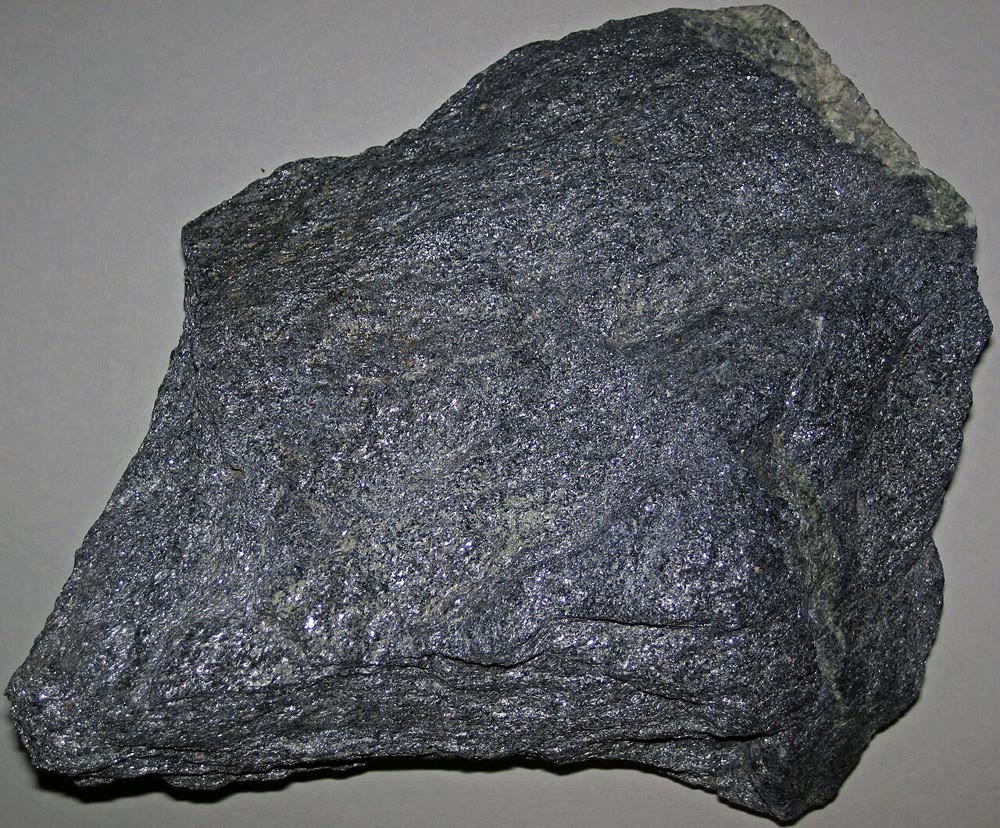
\includegraphics[width=0.27\linewidth]{images/book4/b2-10-blueschist.jpg}\hspace{0.02\linewidth}%
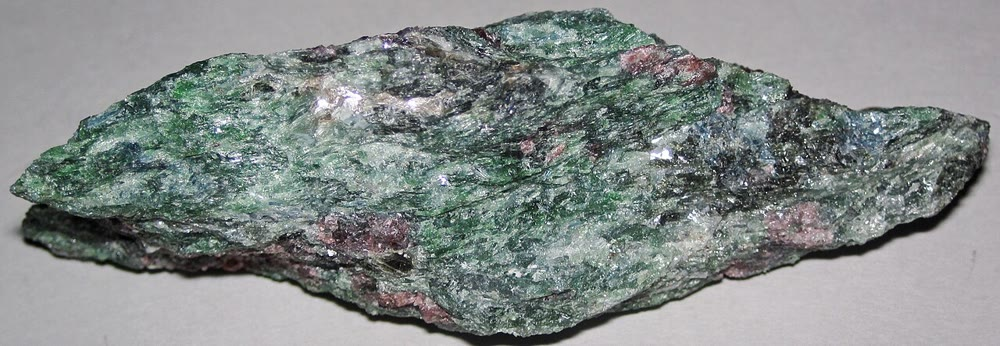
\includegraphics[width=0.69\linewidth]{images/book4/b2-10-eclogite.jpg}
\par\smallskip{\small दो कायांतरित बेसाल्ट। बाएँ: कैलिफ़ोर्निया के फ़्रांसिस्कन संकुल का
एक लॉसनाइट नीलशिस्ट, ग्लॉकोफ़ेन से नीला। दाएँ: पश्चिमी नॉर्वे का एक एक्लोजाइट,
हरा ओम्फ़ैसाइट और लाल गार्नेट, कुछ क्वार्ट्ज़, कायनाइट और रूटाइल के साथ।
फ़ोटो: James St.~John, CC BY 2.0।}
\end{omfigure}

एक साथ दबी और गरम हुई चट्टानें एक नियमित क्रम में संलक्षणियों से गुज़रती हैं, जो
उनके पथ के अनुदिश दाब और तापमान के अनुपात को दर्शाता है: क्षेपण
क्षेत्र में ऊँचा, जहाँ नीलशिस्ट बनते हैं; टक्कर-पट्टी में मध्यम; किसी अंतर्वेधन के निकट निम्न।
\Cref{ch:b2:pt-paths} इन श्रेणियों के नाम बताता है और खनिजों से ऐसे पथ पढ़ता है।
% ledger: scmr:facies

\section{प्रोटोलिथ का महत्त्व}\label{sec:b2:metamorphic-facies:protoliths}

संलक्षणियाँ बेसाल्टों पर परिभाषित हैं, पर हर \omterm{def:b2:metamorphic-facies:metamorphism}{प्रोटोलिथ} उन्हीं परिस्थितियों को
अपने खनिजों में दर्ज करता है।

\begin{definition}[मेटापेलाइट; मेटाबेसाइट]\label{def:b2:metamorphic-facies:protoliths}
\emph{मेटापेलाइट}\index{मेटापेलाइट} एक कायांतरित मडस्टोन (एक पेलाइट) है, जो
ऐलुमिनियम और पोटैशियम में समृद्ध है, और जिसके समुच्चयों में अभ्रक, क्लोराइट, गार्नेट, स्टॉरोलाइट और
ऐलुमिनोसिलिकेट होते हैं। \emph{मेटाबेसाइट}\index{मेटाबेसाइट} एक कायांतरित बेसाल्ट,
गैब्रो या अन्य मैफ़िक चट्टान है, जो कैल्शियम, मैग्नीशियम और लोहे में समृद्ध है, और जिसके समुच्चय
संलक्षणियों को परिभाषित करते हैं।
\end{definition}

\omterm{def:b2:metamorphic-facies:protoliths}{मेटापेलाइट} में पुस्तक 2 के सूचक खनिज \omterm{def:b2:metamorphic-facies:metamorphism}{कायांतरण} श्रेणी बढ़ने के साथ क्रम से प्रकट होते हैं
(क्लोराइट, बायोटाइट, गार्नेट, स्टॉरोलाइट, कायनाइट, सिलिमेनाइट), इस अध्याय की
मस्कोवाइट + क्वार्ट्ज़ अभिक्रिया और भी ऊँचे तापमान पर सिलिमेनाइट और K-फ़ेल्डस्पार बनाती है,
और उपस्थित ऐलुमिनोसिलिकेट बताता है कि चट्टान त्रिक
बिंदु के किस ओर से गुज़री। कायांतरित चूना-पत्थर या डोलोस्टोन संगमरमर बन जाता है, कैल्साइट या
डोलोमाइट का; सिलिका और मृत्तिका वाले अशुद्ध कार्बोनेट कैल्क-सिलिकेट चट्टानें बन जाते हैं, जिनकी
विकार्बनीकरण अभिक्रियाएँ कार्बन डाइऑक्साइड मुक्त करती हैं; क्वार्ट्ज़ बलुआ पत्थर क्वार्ट्ज़ाइट बन जाता है,
जो अपने कण-आकार के सिवा बहुत कम दिखाता है। क्लोराइट क्षेत्र का एक \omterm{def:b2:metamorphic-facies:protoliths}{मेटापेलाइट} और उसके पास का एक
मेटाबेसाल्ट, समान दाब और तापमान पर, बिल्कुल अलग दिखते हैं; दूसरा
ऐक्टिनोलाइट, क्लोराइट, एपिडोट और एल्बाइट का एक हरितप्रस्तर है: परिस्थितियों का एक समूह,
दो समुच्चय।
% ledger: iugs:barrow, day73:ms-qz, scmr:facies-assemblages

\section{अभ्यास}

\begin{exercise}[$\star$]\label{exo:b2:metamorphic-facies:1}
\omterm{def:b2:metamorphic-facies:metamorphism}{कायांतरण} का प्रकार बताइए: (क) एक ग्रेनाइट से
\qty{500}{m} के भीतर संगमरमर में पुनःक्रिस्टलित एक चूना-पत्थर; (ख) किसी बड़े नतिलंब-सर्पण
भ्रंश के अनुदिश एक सूक्ष्म-कणिक, पट्टीदार चट्टान, जिसके कण कुचले और पुनःक्रिस्टलित हुए हैं; (ग) महासागरीय भूपर्पटी का एक बेसाल्ट जिसका
काँच किसी कटक के निकट क्लोराइट और ज़िओलाइटों में बदल गया है, और जिसके खनिज केवल आंशिक रूप से
प्रतिस्थापित हुए हैं; (घ) \qty{10}{km} मोटे ढेर के तल पर ज्वालामुखीय बलुआ पत्थर,
जो शिस्टता के बिना पुनःक्रिस्टलित हुए हैं।
\end{exercise}
% ledger: scmr:types

\begin{exercise}[$\star$]\label{exo:b2:metamorphic-facies:2}
ऐलुमिनोसिलिकेटों की तालिका से $\Delta_r S$, $\Delta_r V$ और \omterm{def:b2:metamorphic-facies:clapeyron}{क्लेपेरॉन ढलान} परिकलित कीजिए,
कायनाइट $\to$ सिलिमेनाइट के लिए, \unit{bar/K} में और \unit{MPa/K} में। \qty{100}{\celsius} में
साम्य-दाब कितना बदलता है?
\end{exercise}
% ledger: rh95:al2sio5

\begin{exercise}[$\star$]\label{exo:b2:metamorphic-facies:3}
हर मेटाबेसाल्ट किस संलक्षणी का है? (क) ऐक्टिनोलाइट, एल्बाइट, क्लोराइट और
एपिडोट; (ख) ग्लॉकोफ़ेन और लॉसनाइट; (ग) हॉर्नब्लेंड और
\qty{30}{\percent} एनॉर्थाइट वाला प्लैजियोक्लेज़; (घ) ओम्फ़ैसाइट और गार्नेट, प्लैजियोक्लेज़ नहीं।
\end{exercise}
% ledger: scmr:facies-assemblages

\begin{exercise}[$\star$]\label{exo:b2:metamorphic-facies:4}
(क) मोलर द्रव्यमान \qty{162.046}{g.mol^{-1}} और मोलर आयतनों 44.15, 51.52 और
\qty{49.86}{cm^3.mol^{-1}} से कायनाइट, ऐंडालुसाइट और सिलिमेनाइट के घनत्व परिकलित कीजिए।
(ख) दाब किसका पक्ष लेता है, और क्यों? (ग) खनिज डेटाबेस 3.61, 3.15 और
\qty{3.24}{g.cm^{-3}} देते हैं: प्राकृतिक क्रिस्टल शुद्ध प्रावस्थाओं से भिन्न क्यों हो सकते हैं?
\end{exercise}
% ledger: rh95:al2sio5, webmineral:polymorphs

\begin{exercise}[$\star\star$]\label{exo:b2:metamorphic-facies:5}
कायनाइट $\to$ ऐंडालुसाइट के लिए $\Delta_r H = \qty{3.9}{kJ}$, $\Delta_r S =
\qty{8.59}{J.K^{-1}}$, $\Delta_r V = \qty{0.737}{J.bar^{-1}}$। (क) \qty{25}{\celsius} और \qty{1}{bar} पर
कौन-सा बहुरूप स्थायी है? (ख) \qty{1}{bar} पर दोनों किस तापमान पर
सहअस्तित्व में होते हैं? (ग) \qty{400}{\celsius} पर साम्य-दाब परिकलित कीजिए और
उसकी तुलना प्रायोगिक \qty{2.54}{kbar} से कीजिए। (घ) फिर भी ऐंडालुसाइट उन चट्टानों में क्यों
मिलता है जो सतह तक ठंडी हो गईं?
\end{exercise}
% ledger: rh95:al2sio5, hm93:table11

\begin{exercise}[$\star\star$]\label{exo:b2:metamorphic-facies:6}
विधि के चरण (2) को परखिए। \qty{1000}{K} पर तालिकाएँ कायनाइट के लिए $S_T$ = 285.02
और सिलिमेनाइट के लिए 296.44 देती हैं, और $(H_T - H_{298})/T$ = 122.29 और 121.39
(\unit{J.mol^{-1}.K^{-1}})। (क) $\Delta_r H$, $\Delta_r S$ और $\Delta_r G$ परिकलित कीजिए,
कायनाइट $\to$ सिलिमेनाइट के, \qty{1000}{K} और \qty{1}{bar} पर। (ख) तालिका के स्थिर
मानों से तुलना कीजिए। (ग) वहाँ कौन-सा बहुरूप स्थायी है, और सरल विधि की
त्रुटि कितनी बड़ी है?
\end{exercise}
% ledger: rh95:al2sio5-ht, rh95:al2sio5

\begin{exercise}[$\star\star$]\label{exo:b2:metamorphic-facies:7}
कैल्साइट और ऐरागोनाइट (\ce{CaCO3}) के, \qty{298.15}{K} पर, $\Delta_f G$ = $-1128.5$ और
$-1127.4$ \unit{kJ.mol^{-1}}, $S$ = 91.7 और 88.0 \unit{J.mol^{-1}.K^{-1}}, $V$ = 36.93
और \qty{34.15}{cm^3.mol^{-1}} हैं, और निर्माण-एन्थैल्पियाँ बराबर हैं। (क)
\qty{25}{\celsius} पर साम्य-दाब ज्ञात कीजिए। (ख) \omterm{def:b2:metamorphic-facies:clapeyron}{क्लेपेरॉन ढलान} परिकलित कीजिए। (ग)
\qty{300}{\celsius} पर साम्य-दाब ज्ञात कीजिए। (घ) अनेक कवच ऐरागोनाइट के बने होते हैं और
\qty{1}{bar} पर जीते हैं: इससे क्या पता चलता है?
\end{exercise}
% ledger: rh95:cc-ar

\begin{exercise}[$\star\star$]\label{exo:b2:metamorphic-facies:8}
एल्बाइट $\to$ जेडाइट + क्वार्ट्ज़ के लिए तालिकाएँ $\Delta_r H = \qty{-5.0}{kJ}$,
$\Delta_r S = \qty{-32.4}{J.K^{-1}}$, $\Delta_r V = \qty{-1.698}{J.bar^{-1}}$ देती हैं। (क)
\omterm{def:b2:metamorphic-facies:clapeyron}{क्लेपेरॉन ढलान} परिकलित कीजिए। (ख) \qty{500}{\celsius} पर साम्य-दाब परिकलित कीजिए।
(ग) एल्बाइट, जेडाइट और क्वार्ट्ज़ की निर्माण-एन्थैल्पियों में 2.6, 3.6
और \qty{1.0}{kJ.mol^{-1}} की अनिश्चितता है; इन्हें स्वतंत्र त्रुटियों के रूप में जोड़ने पर उस
दाब में कितनी अनिश्चितता है? (घ) एक्लोजाइट संलक्षणी में प्लैजियोक्लेज़ क्यों नहीं होता?
\end{exercise}
% ledger: rh95:ab-jd-qz, scmr:facies-assemblages

\begin{exercise}[$\star\star$]\label{exo:b2:metamorphic-facies:9}
मस्कोवाइट + क्वार्ट्ज़ 1, 2 और
\qty{3}{kbar} पर 603, 637 और \qty{662}{\celsius} पर विघटित होता है। (क) हर बिंदु-युग्म के बीच रेखा की ढलान परिकलित कीजिए। (ख) यदि
इस परास में अभिक्रिया की एन्ट्रॉपी मुश्किल से बदलती है, तो पहले अंतराल से दूसरे तक $\Delta_r V$
किस गुणक से सिकुड़ा? (ग) इसके लिए कौन-सी प्रावस्था उत्तरदायी है?
\end{exercise}
% ledger: day73:ms-qz

\begin{exercise}[$\star\star\star$]\label{exo:b2:metamorphic-facies:10}
विधि के स्थिर गुणों के साथ: (क) \qty{600}{\celsius} पर तीनों
अभिक्रियाओं के दाब परिकलित कीजिए; (ख) दिखाइए कि \qty{600}{\celsius} पर और
कायनाइट $=$ ऐंडालुसाइट के दाब पर सिलिमेनाइट सबसे स्थायी बहुरूप है, जिससे रेखा का यह बिंदु
मितस्थायी है; (ग) \qty{600}{\celsius} और
\qty{4}{kbar} पर, और \qty{600}{\celsius} और \qty{7}{kbar} पर कौन-सा बहुरूप स्थायी है?
\end{exercise}
% ledger: rh95:al2sio5

\begin{exercise}[$\star\star\star$]\label{exo:b2:metamorphic-facies:11}
एक शिस्ट में कायनाइट, ऐंडालुसाइट और सिलिमेनाइट एक साथ हैं, तीनों
साम्य में उगे। (क) प्रायोगिक त्रिक बिंदु, $504 \pm \qty{20}{\celsius}$ और
$3.75 \pm \qty{0.25}{kbar}$, और \qty{2700}{kg.m^{-3}} घनत्व वाली भूपर्पटी ($g =
\qty{9.81}{m.s^{-2}}$) के साथ, वह किस गहराई पर उगी? (ख) सतह पर \qty{10}{\celsius} लेते हुए,
इससे किस माध्य ऊष्मीय प्रवणता का संकेत मिलता है? (ग) ऐसी चट्टानें दुर्लभ क्यों हैं?
\end{exercise}
% ledger: hm93:triple

\begin{exercise}[$\star\star\star$]\label{exo:b2:metamorphic-facies:12}
दो चट्टानें गहराई $z$ तक दबाई जाती हैं, सतह पर \qty{10}{\celsius} से शुरू करके: चट्टान X
\qty{10}{\celsius.km^{-1}} के अनुदिश \qty{30}{km} तक, \qty{3000}{kg.m^{-3}} माध्य घनत्व वाली चट्टानों के नीचे,
और चट्टान Y \qty{30}{\celsius.km^{-1}} के अनुदिश \qty{20}{km} तक,
\qty{2800}{kg.m^{-3}} माध्य घनत्व वाली चट्टानों के नीचे। (क) हर पथ के अंत में $T$ और $P$ परिकलित कीजिए।
(ख) स्थिर-गुण रेखाओं के साथ (कैल्साइट $=$ ऐरागोनाइट: $P = 13.31\,T$ बार, जहाँ $T$
केल्विन में; एल्बाइट $=$ जेडाइट + क्वार्ट्ज़ \cref{exo:b2:metamorphic-facies:8} से; ऐलुमिनोसिलिकेट
तालिका से), हर चट्टान में ऐरागोनाइट या कैल्साइट में से कौन, जेडाइट + क्वार्ट्ज़ या एल्बाइट में से कौन, और कौन-सा
ऐलुमिनोसिलिकेट है? (ग) कौन-सा पथ अधिक ठंडा, उच्च-दाब वाला है, और हर एक किस संलक्षणी में समाप्त होता है?
\end{exercise}
% ledger: rh95:cc-ar, rh95:ab-jd-qz, rh95:al2sio5

\section{समस्या: त्रिक बिंदु का निर्माण}

\begin{problem}[{सप्ताहांत समस्या --- तालिकाओं से ऐलुमिनोसिलिकेट आरेख, और उस पर कितना
भरोसा किया जाए}]
\label{pb:b2:metamorphic-facies:1}
ऐलुमिनोसिलिकेटों की तालिका (\qty{298.15}{K}, \qty{1}{bar}) और इस अध्याय की विधि का
उपयोग कीजिए, स्थिर $\Delta_r H$, $\Delta_r S$ और $\Delta_r V$ के साथ; $T$ को
केल्विन में, $P$ को बार में लिखिए, और $P - 1$ में 1 की उपेक्षा कीजिए।

\noindent\textbf{भाग I --- अभिक्रियाएँ।}
\begin{enumerate}
\item $\Delta_r H$, $\Delta_r S$ और $\Delta_r V$ परिकलित कीजिए, कायनाइट $\to$ ऐंडालुसाइट के लिए।
\item कायनाइट $\to$ सिलिमेनाइट के लिए भी यही कीजिए।
\item ऐंडालुसाइट $\to$ सिलिमेनाइट के लिए भी यही कीजिए, और जाँचिए कि हर गुण
पहले दो का अंतर है।
\item किस बहुरूप की एन्ट्रॉपी सबसे अधिक है, किसका आयतन सबसे कम? हर रेखा के किस ओर
कौन-सा स्थित होगा?
\item तीनों क्लेपेरॉन ढलानें परिकलित कीजिए।
\item ऐंडालुसाइट $\to$ सिलिमेनाइट की ढलान ऋणात्मक क्यों है?
\end{enumerate}

\noindent\textbf{भाग II --- रेखाएँ कहाँ से गुज़रती हैं।}
\begin{enumerate}[resume]
\item \qty{298.15}{K} पर पहली दो अभिक्रियाओं का $\Delta_r G$ परिकलित कीजिए। सतह पर कौन-सा
बहुरूप स्थायी है?
\item \qty{1}{bar} पर हर अभिक्रिया किस तापमान (\unit{\celsius} में) पर
साम्य में पहुँचती है?
\item प्रश्न~8 के तीन तापमानों में से कौन-से स्थायी साम्य हैं और कौन-से
मितस्थायी? (\qty{1}{bar} पर तीनों के क्रम का उपयोग कीजिए।)
\item \qty{400}{\celsius} पर कायनाइट $=$ ऐंडालुसाइट का दाब परिकलित कीजिए;
प्रयोग \qty{2.54}{kbar} देते हैं।
\item \qty{700}{\celsius} पर कायनाइट $=$ सिलिमेनाइट का दाब परिकलित कीजिए;
प्रयोग \qty{7.86}{kbar} देते हैं।
\item 200 और \qty{900}{\celsius} के बीच तीनों रेखाओं का रेखाचित्र बनाइए।
\end{enumerate}

\noindent\textbf{भाग III --- त्रिक बिंदु।}
\begin{enumerate}[resume]
\item पहली दो रेखाओं को $P = a_i T - b_i$ के रूप में लिखिए; $a_1$, $b_1$, $a_2$, $b_2$ बताइए।
\item उनके प्रतिच्छेद का तापमान हल कीजिए।
\item उसका दाब परिकलित कीजिए।
\item जाँचिए कि ऐंडालुसाइट $=$ सिलिमेनाइट उससे होकर जाती है।
\item प्रायोगिक $504 \pm \qty{20}{\celsius}$ और $3.75 \pm
\qty{0.25}{kbar}$ से तुलना कीजिए।
\item तालिकाओं की तापमान-निर्भरता के साथ त्रिक बिंदु
\qty{536}{\celsius} और \qty{4.20}{kbar} पर खिसक जाता है। क्या परिष्करण ने उसे
प्रयोग के निकट लाया? इससे त्रुटि के मुख्य स्रोत के बारे में क्या संकेत मिलता है?
\end{enumerate}

\noindent\textbf{भाग IV --- उस पर कितना भरोसा करें।}
\begin{enumerate}[resume]
\item ऐंडालुसाइट की निर्माण-एन्थैल्पी \qty{1}{kJ} बढ़ाइए। स्थिर तापमान पर
कायनाइट $=$ ऐंडालुसाइट रेखा दाब में कितनी खिसकती है?
\item त्रिक बिंदु तापमान में कितना खिसकता है?
\item सिलिमेनाइट की एन्थैल्पी में \qty{1}{kJ} की वृद्धि के लिए भी यही कीजिए।
\item हर एन्थैल्पी में \qty{2.0}{kJ} की अनिश्चितता है। अकेले कैलोरीमितीय आँकड़े त्रिक बिंदु के
तापमानों का कौन-सा परास अनुमत करते हैं?
\item तब ऊष्मागतिक तालिकाएँ प्रायोगिक आरेख को
\qty{30}{\celsius} के भीतर कैसे पुनः उत्पन्न कर सकती हैं?
\item भाग III में परिकलित त्रिक बिंदु का तापमान, अंश तक पूर्णांकित, बताइए:
यह इस समस्या की मुख्य संख्या है।
\end{enumerate}
\end{problem}
% ledger: rh95:al2sio5, rh95:al2sio5-ht, hm93:triple, hm93:table11, hm93:adjusted
